\section{Flow matching with the path-integral method fails on a circular dataset}

We have shown that flow matching with a path integral works well for high-dimensional, non-circular data. To compute the Hellinger distance between $\theta_i$ and $\theta_j$, one integrates along $\theta$ between indices $i$ and $j$. This is unproblematic when the stimulus is not periodic; for circular stimuli, however, the path integral can take ``detours'' that accumulate error along the path and degrade the Hellinger-distance estimate.

Here we ask whether flow matching with path-integral estimation still performs well on a circular dataset. We constructed such a dataset from cosine tuning curves, with independent observation noise whose variance scales linearly with the absolute firing rate (conditional mean). The cosine period is $2\pi$; we intentionally took $\theta$ from $-6$ to $6$ so that the interval spans roughly two periods (see Methods for dataset details, figure \ref{fig:circular_dataset}A and C).

We applied the same flow-matching path-integral procedure to estimate the Hellinger RDM. The estimator failed to respect the circular structure of the stimulus (figure \ref{fig:circular_dataset}B and D).

\begin{figure}[H]
  \centering
  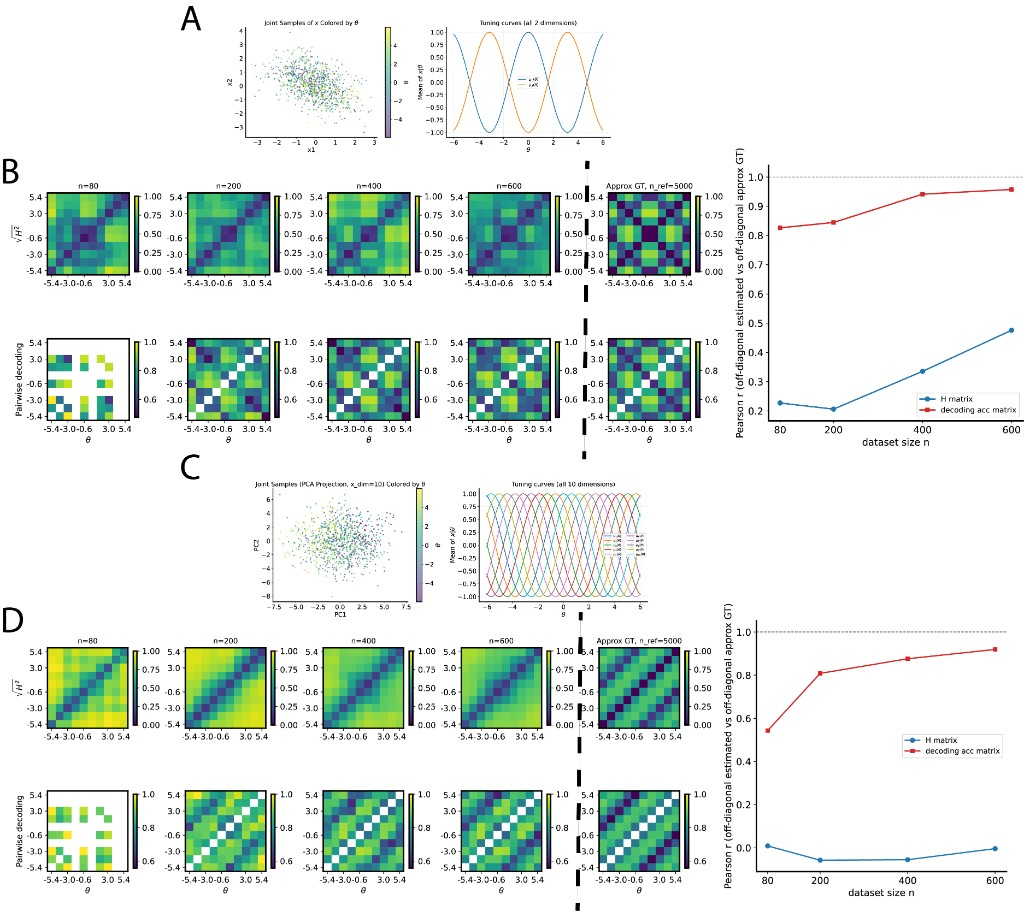
\includegraphics[width=\linewidth]{notes/figures/path-integral-failure/circular_dataset_jointviz_h_vs_decoding.png}
  \caption{Cosine circular data and estimates for $d=2$ (A--B) and $d=10$ (C--D). \textbf{A,C:} joint samples of $x$ (PCA projection in 10D) colored by $\theta$, and tuning curves across dimensions. \textbf{B,D:} heatmaps of $\sqrt{H^2}$ from path-integral estimation versus pairwise decoding accuracy across training set sizes $n$; curves show Pearson $r$ between off-diagonal entries and the reference.}
  \label{fig:circular_dataset}
\end{figure}


\subsection{Methods: Cosine dataset}
We use a synthetic conditional model for a scalar stimulus $\theta$ and a multivariate observation $x \in \mathbb{R}^{d}$ with $d \ge 2$.
Stimuli are drawn independently from a uniform density on a bounded interval,
\begin{equation}
  \theta \sim \mathrm{Uniform}(\theta_{\mathrm{low}}, \theta_{\mathrm{high}}).
\end{equation}

\paragraph{Conditional mean (tuning curve).}
For each coordinate $j \in \{1,\ldots,d\}$, fix a phase $\phi_j = 2\pi(j-1)/d$.
Given $\theta$, the mean of $x_j$ is a cosine in $\theta$,
\begin{equation}
  \mu_j(\theta) = A \cos(\omega \theta + \phi_j),
  \qquad j = 1,\ldots,d,
\end{equation}
with amplitude $A > 0$ and frequency $\omega > 0$ on the stimulus axis (in the default bundle, $A=\omega=1$).
The conditional mean vector is $\mu(\theta) = (\mu_1(\theta),\ldots,\mu_d(\theta))^{\mathsf{T}}$.

\paragraph{Observation noise.}
Conditionally on $\theta$, the observation is multivariate Gaussian with diagonal covariance.
Let $\sigma_{\mathrm{base},j}>0$ be positive baseline scales across neurons; in the usual configuration they interpolate linearly in $j$ between fixed $\sigma_{1}$ and $\sigma_{2}$, and often $\sigma_{1}=\sigma_{2}=\sigma$ so all coordinates share the same~$\sigma$.
Let $\alpha$ be a fixed activity--variance coupling strength (the arithmetic mean of two nonnegative hyperparameters in the implementation), and let $\varepsilon>0$ be a negligible variance floor.
The per-neuron conditional variances are
\begin{equation}
  v_j(\theta)
  = d\,\sigma_{\mathrm{base},j}^{2}\,\bigl(1 + \alpha\,|\mu_j(\theta)|\bigr) + \varepsilon,
  \qquad j = 1,\ldots,d,
\end{equation}
with independence across neurons,
\begin{equation}
  x \mid \theta \sim \mathcal{N}\!\bigl(\mu(\theta),\,\mathrm{diag}(v_1(\theta),\ldots,v_d(\theta))\bigr).
\end{equation}
Thus noise magnitude increases with $|\mu_j(\theta)|$, and each neuron's noise standard deviation scales proportionally to $\sqrt{d}$ for fixed $\sigma_{\mathrm{base},j}$, $\alpha$, and $\mu_j(\theta)$.
The leading factor~$d$ matches the ``$\sqrt{d}$ noise scaling'' construction used elsewhere in these notes: as $d$ grows, per-coordinate variance grows with~$d$ so that dimension alone does not drive the observation toward an effectively noiseless, trivially informative regime for~$\theta$.